\documentclass[letterpaper, 14pt]{article}
\usepackage[english]{babel}
\usepackage[utf8]{inputenc}
\usepackage{geometry}
\geometry{scale=0.8}
\usepackage{setspace}
\linespread{1.2}

\usepackage{indentfirst}
\usepackage{framed}
\usepackage{enumitem}
\usepackage{array}
\usepackage{bookmark}
\usepackage{tabularx}

\usepackage{hyperref}
\hypersetup{
    colorlinks=true,
    linkcolor=magenta,     
    urlcolor=cyan,
}

\usepackage{amsmath}
\usepackage{amssymb}
\usepackage{mathptmx}

\usepackage{graphicx}
\graphicspath{{Figures/}}
\usepackage{float}
\usepackage{caption}
\usepackage{subcaption}
\usepackage{tikz}
\usetikzlibrary{graphs, automata, positioning, arrows.meta}
\tikzset{
	node distance=2cm, 
	every state/.style={semithick, fill=gray!10},
	initial text={}, 
	double distance=2pt,
	every edge/.style={draw,->,>=stealth',auto,semithick}
}

\usepackage{algorithm}
\usepackage[noend]{algpseudocode}

\usepackage{listings}
\usepackage{courier}
\usepackage{color}
\definecolor{mygreen}{rgb}{0, 0.6, 0}
\lstset{
	backgroundcolor = \color{white},
	basicstyle=\footnotesize\ttfamily, 
	breakatwhitespace = false,
	breaklines = true,
	captionpos = none,
	commentstyle = \color{mygreen},
	frame = single, 
	keepspaces = true, 
	keywordstyle = \color{blue},
	language = Java, 
	numbers = left, 
	numbersep = 5pt, 
	numberstyle = \tiny\color{purple}, 
	rulecolor = \color{black},
	showtabs = false, 
	stepnumber = 1, 
	tabsize = 4, 
	title = \lstname
}


\begin{document}
\title{CS179E: Project in Computer Science -- Compiler\\ Document for Phase 1}
\author{Jiamin Pan, Yunqing Xiao}
\date{}
\maketitle

\section{Introduction}

MiniJava is a subset of Java including most of basic features of Java. \cite{homepage}
In phase 1 of the whole project, we will focus on writing a type checker for MiniJava 
with the parser for MiniJava and some visitor interfaces provided. In this document,
we will explain the details of our design and make a brief review for phase 1. 

\section{Method for Program Design}

Type-checking of a MiniJava program proceeds in two phases. First, we build the symbol table, and then we type-check the statements and expressions. \cite{book} We used to believe that we can combine symbol table construction and type-checking into only one traverse, however it is impossible. Because, in Java and MiniJava, the classes are mutually recursive, and a method can return only one type of values, which makes it difficult to achieve this goal. If we tried to do type-checking in a single phase, then we might need to type-check a call to a method that is not yet entered into the symbol table. Therefore, we also separate the implement for phase 1 into two sub-phases: symbol table construction and type-checking. 

\subsection{Symbol Table Construction}

\subsubsection{Package \texttt{symbol}}

There are a lot of ideas for symbol table construction. For example, we can create a stack including
scopes like classes and methods. We can also use binary trees instead of hash table to make searching
more efficient. In our program, inspired by Cole Fichter, \cite{link} we utilize a hierarchical 
pattern for symbol table design. The idea is illustrated in the following figure. 
\begin{figure}[H]
\centering
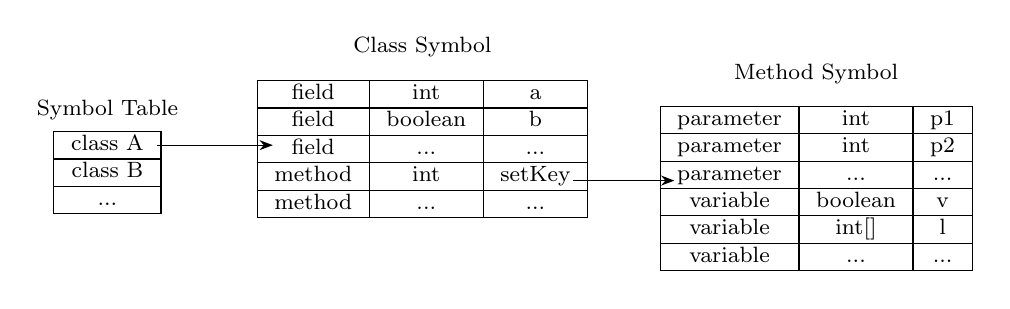
\begin{tikzpicture}[font=\footnotesize]
\node at (0,0) {Symbol Table};
\node at (0,-0.8) {\begin{tabular}{|c|}
\hline class A \\
\hline class B \\
\hline ... \\ \hline
\end{tabular}};

\node at (4,0.8) {Class Symbol};
\node at (4,-0.5) {\begin{tabular}{|c|c|c|}
\hline field & int & a \\
\hline field & boolean & b \\
\hline field & ... & ... \\
\hline method & int & setKey \\
\hline method & ... & ... \\ \hline
\end{tabular}};

\node at (9,0.45) {Method Symbol};
\node at (9,-1) {\begin{tabular}{|c|c|c|}
\hline parameter & int & p1 \\
\hline parameter & int & p2 \\
\hline parameter & ... & ... \\
\hline variable & boolean & v \\
\hline variable & int[] & l \\
\hline variable & ... & ... \\ \hline
\end{tabular}
};

\draw[-{Stealth}] (0.625,-0.45) -- (2.1,-0.45);
\draw[-{Stealth}] (5.91,-0.9) -- (7.2,-0.9);
\end{tikzpicture}
\caption{Hierarchical Symbol Table}
\end{figure}

We maintain a symbol table containing all the symbol of classes. For each class, 
it contains all the fields and methods, and each method contains all the parameters
and local variables. This idea is easy to be implemented, since we can create a base
class \texttt{Symbol} and extend it to get adapted to different conditions. These classes
are contained in a package \texttt{symbol}. 
\begin{figure}[H]
\centering
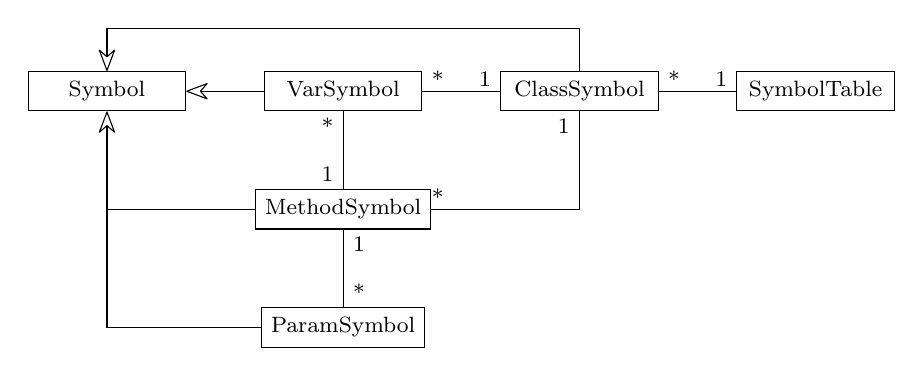
\begin{tikzpicture}[font=\footnotesize]
\node (symbol) [minimum width=2cm, minimum height=0.5cm,draw] at (0,0) {Symbol};
\node (vars) [minimum width=2cm, minimum height=0.5cm,draw] at (3,0) {VarSymbol};
\node (cls) [minimum width=2cm, minimum height=0.5cm,draw] at (6,0) {ClassSymbol};
\node (st) [minimum width=2cm, minimum height=0.5cm,draw] at (9,0) {SymbolTable};
\node (mtds) [minimum width=2cm, minimum height=0.5cm,draw] at (3,-1.5) {MethodSymbol};
\node (pms) [minimum width=2cm, minimum height=0.5cm,draw] at (3,-3) {ParamSymbol};
\draw[-{Stealth[length=3mm, open, round]}] (vars) -- (symbol);
\draw[-{Stealth[length=3mm, open, round]}] (mtds) -| (symbol);
\draw (pms) -| (0,-1.5);
\draw (cls) |- (0,0.8);
\draw[-{Stealth[length=3mm, open, round]}] (0,0.8) -- (symbol);
\draw (vars) -- (mtds); \draw (vars) -- (cls); 
\draw (pms) -- (mtds); \draw (mtds) -| (cls);
\draw (cls) -- (st);
\node at (2.8,-1.05) {1}; \node at (2.8,-0.45) {*};
\node at (3.2,-1.95) {1}; \node at (3.2,-2.55) {*};
\node at (4.2, 0.15) {*}; \node at (4.8, 0.15) {1};
\node at (4.2, -1.35) {*}; \node at (5.8, -0.45) {1};
\node at (7.2, 0.15) {*}; \node at (7.8, 0.15) {1};
\end{tikzpicture}
\caption{Relationship between Classes in package \texttt{symbol}}
\end{figure}

The code below is a sketch for \texttt{SymbolTable.java}. Notice that we create an instance of \texttt{HashMap} to record all classes. Moreover, we simply define a method \texttt{findClass()} to obtain the class record we want instead of directly calling the \texttt{find()} method of \texttt{HashMap}, because we need to keep the encapsulation of our class. 
\begin{lstlisting}
// Class for final symbol table
public class SymbolTable {
	private HashMap<String, ClassSymbol> cls;	// List of classes
	
	......
	
	// Find class from the list
	public ClassSymbol findClass(String _name) {
		return this.cls.get(_name);
	}
	
	......
}
\end{lstlisting}

The implementation of other classes is similar. However, we also need to clarify the inheritance of classes. We can add a field \texttt{baseClass} for each class and set it \texttt{null} if this class does not extend others. Besides, the \texttt{findField()} method and \texttt{findMethod()} method of \texttt{ClassSymbol} should deal with this problem. By the code below, we directly return the value as long as we can find a matching result in current class. Only when we find no matches in current class shall we turn to search the base classes. 
\begin{lstlisting}
// Find a matching field
public VarSymbol findField(String _name) {
	if (this.flds.containsKey(_name)) {
		return this.flds.get(_name);
	} else if (this.baseClass != null) {
		return this.baseClass.findField(_name);
	} else {
		return null;
	}
}
\end{lstlisting}

\subsubsection{Traversing Source Code}

Then what we need to do next is to traverse the source code file and construct the symbol table. Remember that we have a type system for MiniJava, so we will create a visitor to visit these nodes and accept them if they observe the rules in type system. 

Here we use \texttt{GJNoArguVisitor<R>} interface and set \texttt{R} to be \texttt{String}, because we let each record for either names or types to be a string so the whole symbol table will not occupy too much resources. We also add two fields \texttt{currClass} and \texttt{currMethod} to record current scope, as we visit each node
by recursion. Once we set current scope, then it will also be adapted to all the nodes within it. 
\begin{lstlisting}
// Vistor for building symbol table
public class BuildSTVisitor implements GJNoArguVisitor<String> {
	private SymbolTable sTable;			// General Symbol table for all classes
	......
	private ClassSymbol currClass;		// Used during construction, record current class
	private MethodSymbol currMethod;	// Used during construction, record current method

	......

	public String visit(Identifier n) {
		return n.f0.accept(this);
	}
	
	......
}
\end{lstlisting}

Then we will visit the declaration of classes. We can refer to the code below such that the \texttt{visit} method will return the string of identifier as long as our visitor visits an identifier. Hence, we first obtain the name of class and check whether it is already in the table. If it is in symbol table, then we will not accept the remain 
nodes since we cannot let two classes have the same name; otherwise, we create a instance of \texttt{ClassSymbol} for this class and allocate it to \texttt{currClass}. Then the following nodes will be within the scope of \texttt{currClass}. After we have traversed the fields and methods of current scope, we set \texttt{currClass} to be \texttt{null} so it will be reused in the following classes. 
\begin{lstlisting}
public String visit(ClassDeclaration n) {
	String _ret=null;
	n.f0.accept(this);
	String className = n.f1.accept(this);
	ClassSymbol _class = this.sTable.addClass(className);
	if (_class == null) {
		this.error.complain("The class " + className + " has already been defined!");
	} else {
		setCurrentClass(_class);
		n.f2.accept(this); n.f3.accept(this);
		n.f4.accept(this); n.f5.accept(this);
		setCurrentClass(null);
	}
	return _ret;
}
\end{lstlisting}

Similarly, when the visitor visit a method, it will also set \texttt{currMethod} to be current method symbol and reset it after we have traversed the whole method. However, what we also need to pay attention to is the declaration of variables. Since it could a field or a local variable. We need to make a choice by the conditions. The code below implements the general idea: When our visitor visits a variable declaration, we get its type and name by the identifiers and check its existence in current scope. Note that for each \texttt{Type} we directly return a string of its type, for example, ``int'' and ``boolean''. As long as we repeat the steps aboves, we will finally obtain a symbol table for the source file. 
\begin{lstlisting}
public String visit(VarDeclaration n) {
	String _ret=null;
	String type = n.f0.accept(this);
	String name = n.f1.accept(this);
	n.f2.accept(this);
	if (currMethod == null) {	// it is a field
		if (!this.currClass.addField(name, type)) {
			this.error.complain("This variable " + name + " has already been defined in class " 
				+ this.currClass.getName());
		}
	} else if (!this.currMethod.addVar(name, type)) {	// it is a local variable
		this.error.complain("This variable " + name + " has already been defined in method " 
			+ this.currMethod.getName() + " of " + this.currClass.getName());
	}
	return _ret;
}
\end{lstlisting}


We take 
\texttt{Factorial.java} for example. 
\begin{lstlisting}
class Factorial{
    public static void main(String[] a){
        System.out.println(new Fac().ComputeFac(10));
    }
}

class Fac {
    public int ComputeFac(int num){
        int num_aux ;
        if (num < 1)
            num_aux = 1 ;
        else
            num_aux = num * (this.ComputeFac(num-1)) ;
        return num_aux ;
    }
}
\end{lstlisting}

The symbol table will be like this:
\begin{figure}[H]
\centering
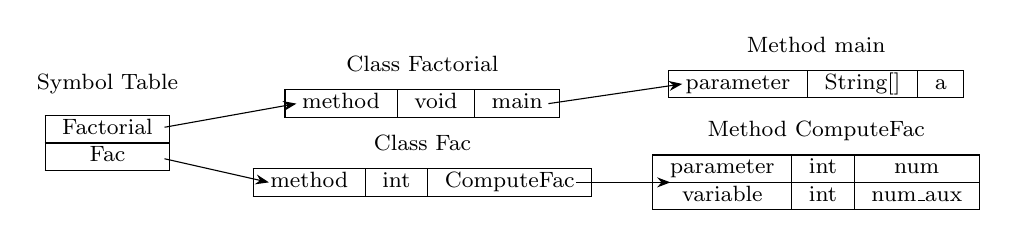
\begin{tikzpicture}[font=\footnotesize]
\node at (0,0) {Symbol Table};
\node at (0,-0.75) {\begin{tabular}{|c|}
\hline Factorial \\
\hline Fac \\ \hline
\end{tabular}};

\node at (4,0.25) {Class Factorial};
\node at (4,-0.25) {\begin{tabular}{|c|c|c|}
\hline method & void & main \\ \hline
\end{tabular}};

\node at (4,-0.75) {Class Fac};
\node at (4,-1.25) {\begin{tabular}{|c|c|c|}
\hline method & int & ComputeFac \\ \hline
\end{tabular}};

\node at (9,0.5) {Method main};
\node at (9,0) {\begin{tabular}{|c|c|c|}
\hline parameter & String[] & a \\ \hline
\end{tabular}
};

\node at (9,-0.6) {Method ComputeFac};
\node at (9,-1.25) {\begin{tabular}{|c|c|c|}
\hline parameter & int & num \\ 
\hline variable & int & num\_aux \\ \hline
\end{tabular}
};

\draw[-{Stealth}] (0.725,-0.55) -- (2.4,-0.25);
\draw[-{Stealth}] (0.725,-0.95) -- (2.05,-1.25);
\draw[-{Stealth}] (5.6,-0.25) -- (7.3,0);
\draw[-{Stealth}] (5.95,-1.25) -- (7.15,-1.25);
\end{tikzpicture}
\caption{Symbol Table for \texttt{Factorial.java}}
\end{figure}

\subsection{Type-Checking}

\subsubsection{Deciding Symbol's Type}

Then we go to the phase for type-checking. We can send the symbol table we built in last phase to the new visitor so that it will be able to use symbol table to check each identifier's type. Just like what we did in last phase, we directly return the string of an identifier, which simplifies the comparison of records since we just need to call \texttt{String.equals(s)}. However, the string we get could be either a type or name of some variables. We should clarify them and finally determine its type. 

Hence, we add a method \texttt{getIDType} to solve the problem. If it is a built-in type, we just return it; otherwise, we try finding it in classes and methods in symbol table. As long as we can find a matching record, we directly return its type. The sketch of implementation is listed below. We will use this method to get the types in the following traversing process. 
\begin{lstlisting}
// Return the type of an identifier
private String getIDType(String _name) {
	String type = null;
	if (_name != null) {
		if (_name.equals("int") || _name.equals("boolean") || _name.equals("int[]") 
			|| this.sTable.findClass(_name) != null) {	// If the string is a type
			type = _name;
		} else {	// Then the string is a name
			if (this.currMethod == null) {	// If it is a field
				VarSymbol var = this.currClass.findField(_name);
				if (var == null) {
					setError(true);
				} else {
					type = var.getType();
				}
			} else {	// If it is in a method
				ParamSymbol param = this.currMethod.findParam(_name);
				VarSymbol var_mtd = this.currMethod.findVar(_name);
				if (param == null && var_mtd == null) {
					setError(true);
				} else if (param != null) {	// It is a parameter
					type = param.getType();
				} else if (var_mtd != null) {	// It is a variable
					type = var_mtd.getType();
				}
			}
		}
	}
	return type;
}
\end{lstlisting}

\subsubsection{Visiting Source Code}

Since we can obtain the types by the method \texttt{getIDType} above, we just need to visit each node and check whether it matches the record in symbol table. For example, we can deal with \texttt{AndExpression} and \texttt{PlusExpression} like this. 
\begin{lstlisting}
public String visit(AndExpression n) {
	String _ret = "boolean";
	String leftType = getIDType(n.f0.accept(this));
	n.f1.accept(this);
	String rightType = getIDType(n.f2.accept(this));
	if (!leftType.equals("boolean") || !rightType.equals("boolean")) {
		setError(true);
	}
	return _ret;
}

......

public String visit(PlusExpression n) {
	String _ret="int";
	String leftType = getIDType(n.f0.accept(this));
	n.f1.accept(this);
	String rightType = getIDType(n.f2.accept(this));
	if (!leftType.equals("int") || !rightType.equals("int")) {
		setError(true);
	}
	return _ret;
}
\end{lstlisting}

We just return the type of expression by the type of ``value'' of it. This choice makes it easier in other type-checking, for example, \texttt{println(e)}. If we can get the type of \texttt{e}, then we just need to check whether it matchs ``int''. Applying this idea to the whole visitor, we can accomplish almost all type-checking. 

\subsubsection{How to Visit \texttt{instance.method(arg1,...)}}

At the first glance, the problem seems to be settled. However, here comes another problem. How can we deal with the call for methods by an instance of class, like \texttt{a.getKey(m,n)}? It is easy to check the existence of instance and method, but oppositely, it is hard to determine the number and type of parameters since we use recursion instead of iteration to visit the nodes. 

I have come up with an idea by adding some supporting methods like this:
\begin{lstlisting}
// Return an arraylist containing an array of types of arguments
private ArrayList<String> exprListVisit(NodeOptional n) {
	ArrayList<String> typelist = new ArrayList<String>();
	if (n.present()) {
		if (n.node instanceof ExpressionList) {
			ExpressionList list = (ExpressionList) n.node;
			typelist.add(getIDType(list.f0.accept(this)));
			NodeListOptional restList = (NodeListOptional) list.f1;
			if (restList.present()) {
				for ( Enumeration<Node> e = restList.elements(); e.hasMoreElements(); ) {
					typelist.add(getIDType(e.nextElement().accept(this)));
				}
			}
		}
	}
	return typelist;
}
\end{lstlisting}

By the method above, we just simulate the visit process of expression list and use a \texttt{ArrayList} recording all the arguments' types so that we will be able to determine the number of arguments we use in source code and their types. Since it is easy to verify the number and types of arguments in declaration the method, we can just make another \texttt{ArrayList} recording them by a built-in method \texttt{getTypeList()} and compare the two lists. Note that we will also need to deal with the inheritance since we can pass a subclass instance to a method whose parameter's type is baseclass.  
\begin{lstlisting}
// Check two types are the same or not (or one type inherits from another one)
private boolean isEquivType(String argType, String paraType) {
	if (paraType.equals("int") || paraType.equals("boolean") || paraType.equals("int[]")) {
		return argType.equals(paraType);	// Built-in types, just compare them
	} else {	// Classes, check inheritance
		if (argType.equals(paraType)) {
			return true;
		} else {
			ClassSymbol baseType = this.sTable.findClass(argType).getBaseClass();
			while (baseType == null) {
				if (baseType.getName() == paraType) {
					return true;
				} else {
					baseType = baseType.getBaseClass();
				}
			}
			return false;
		}
	}
}
\end{lstlisting}

\section{Review for Phase 1}
\subsection{The running output of tester}
\begin{lstlisting}
==== Results ====
- Valid Cases: 9/9
- Error Cases: 9/9
- Submission Size = 43 kB
\end{lstlisting}

We have passes all the cases and do not make our code so ``bloated''. The 
result is satisfying but more test cases are still in need. Software testing
is always on the road. 

\subsection{Suggestion for Code Design}

Though I have stated almost all the ideas about the design, I still want to mention
some principles of object-oriented programming (OOP) since I found some codes of interfaces
did not obey them very well. Somehow we can improve it so we could avoid 
some other ``accidents''. 

Java is not like C++. In C++, we always declare a field of one class to be public. However, 
it is suggested to declare all fields of a class to be private and build ``getter'' and 
``setter'' methods to return or modify its value. Therefore, in my codes, I declared all fields
to be private. As long as I need to get access to its value, I will build a ``getter'' to return 
its value. This can make sure we will not visit the fields directly through an instance, which might 
bring potential risks such that anybody would like to modify the value of any field to make it invalid. 
If we can apply this idea to the construction of compiler, it will be much safer than before. 

\begin{thebibliography}{9}

\bibitem{homepage}
	Course's Homepage: 
	\href{https://www.cs.ucr.edu/~lesani/teaching/cp/cp.html}{Compiler Project}. 

\bibitem{book}
	Andrew W. Appel, Jens Palsberg, 
	\textit{Modern Compiler Implementation in Java},
	Cambridge University Press, 
	Second Edition, 
	2002. 

\bibitem{link}
	Cole Fichter, 
	Github Repository: \href{https://github.com/colefichter/Tiger-Compiler}{Tiger-Compiler}. 
	
\bibitem{type}
	Jens Palsberg, 
	\textit{The MiniJava Type System}, 
	2011. 

\end{thebibliography}

\end{document}
